\section{Additional Experimental Results}



\paragraph{Per-Dimension Stability.}
Tab.~\ref{table:stability_analysis} reports the overall stability; here we further break down the analysis by individual evaluation dimensions. As shown in Tab.~\ref{tab:stability_per_dim}, CV remains below 3.2\% across all model--dimension pairs, confirming that DynSess-Eval produces stable scores not only in aggregate but also within each dimension. Notably, \textit{Role Consistency} exhibits the lowest average CV (1.75\%), likely because persona adherence is relatively objective and less susceptible to stochastic variation, whereas \textit{Human-Likeness} shows slightly higher CV (2.35\%), reflecting the inherent subjectivity of this dimension.



\subsection{Inter-Annotator Agreement}
\label{app:iaa}
To verify the reliability of human annotations, we assess inter-annotator agreement at both the model level and the sample level. Three annotators independently score sessions from the 10 models evaluated in Tab.~\ref{tab:model-performance-human} across the 100 test personas.

At the model level, we compute pairwise Pearson correlation coefficients on the averaged model scores (Tab.~\ref{tab:annotator_agreement}) and Spearman rank correlation on the model rankings (Tab.~\ref{tab:annotator_spearman}). All Pearson correlations exceed 0.8 and all Spearman correlations exceed 0.78 with $p < 0.05$, indicating strong and statistically significant agreement on model-level quality assessment.

At the individual sample level, pairwise correlations are naturally lower due to the inherent subjectivity of role-playing evaluation. Nevertheless, all pairwise comparisons yield $p < 10^{-9}$, confirming systematic non-random agreement even at the fine-grained sample level. The moderate sample-level correlations are consistent with prior work on subjective NLG evaluation, and the strong model-level agreement demonstrates that individual variations cancel out upon aggregation.



% 分析讨论单轮RL和多轮RL训练效果的差异，单轮dpo训练过程中loss也下降，但是整体的









% --------0522 RJN 稳定性分析改成表格的形式
% \begin{figure*}[t]
%   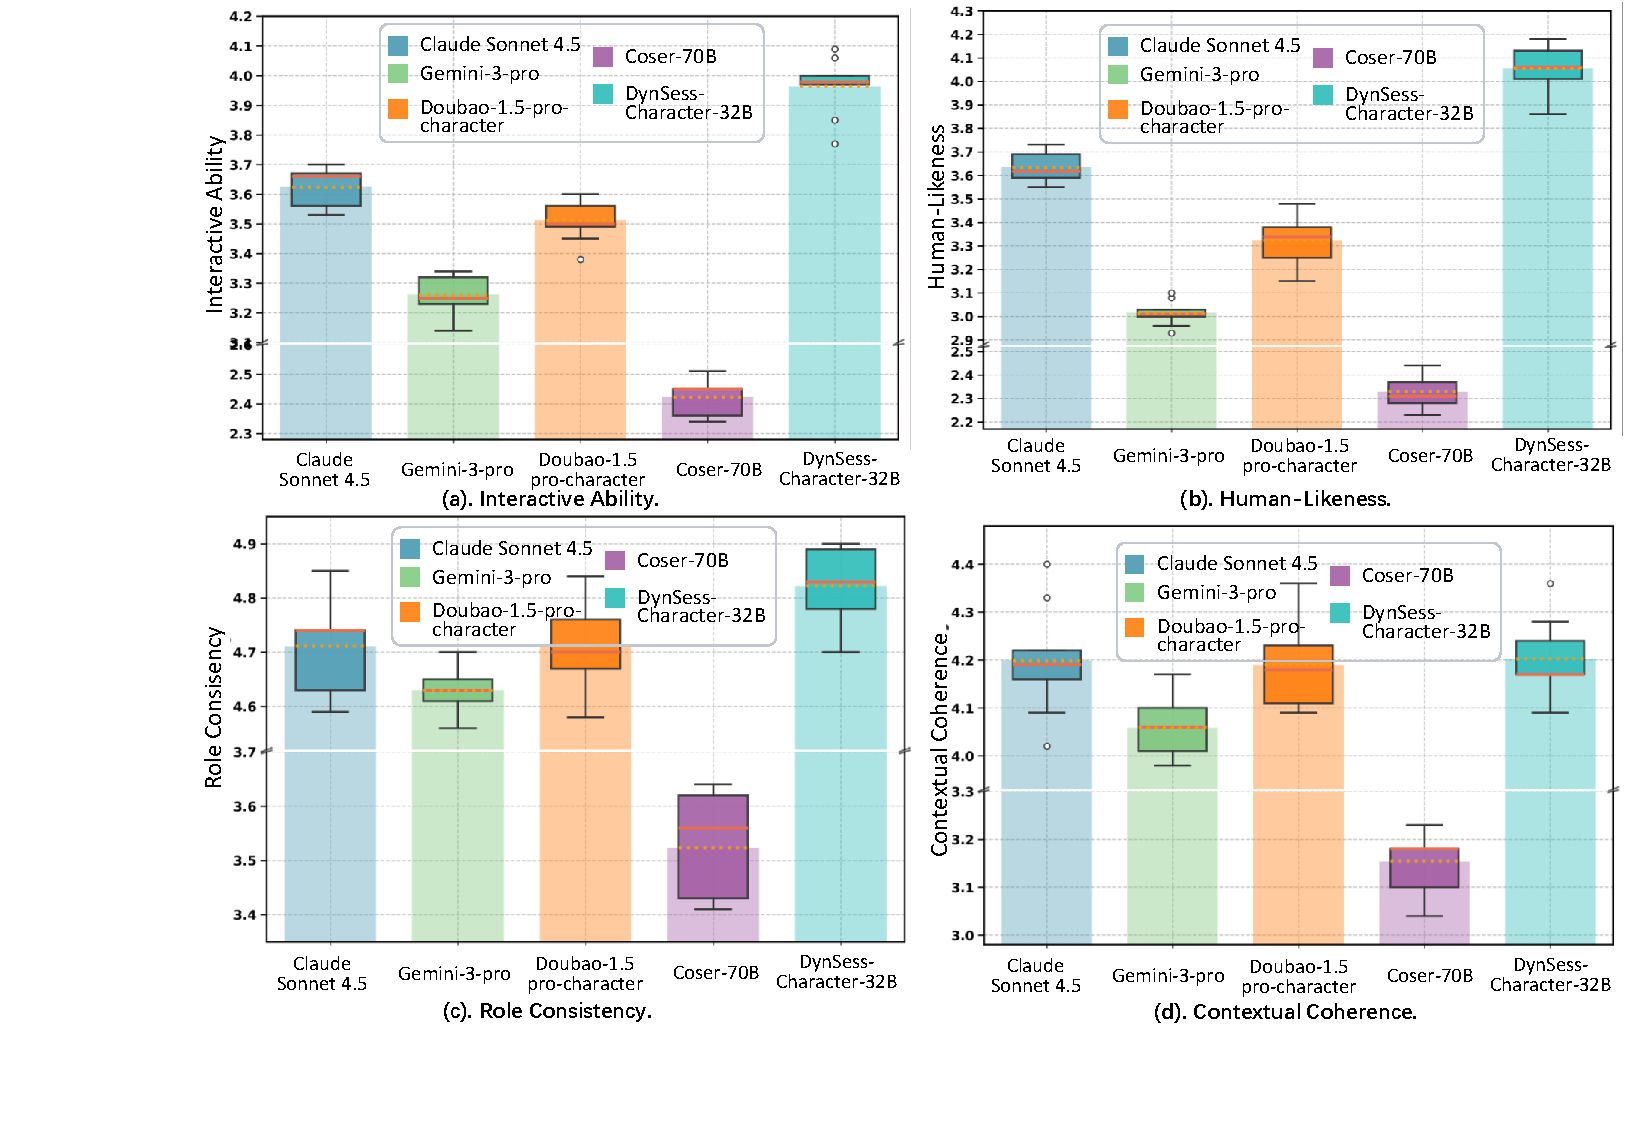
\includegraphics[width=\textwidth, trim = 3.2cm 1cm 0 0, clip]{latex/Image/appendix-experiment-analysis-bias-v2.pdf}

%   \caption{Stability Analysis in Four Dimensions.}
%   \label{fig:experiments}
% \end{figure*}


% \subsection{Response Length Analysis}

% To examine whether response length introduces bias in evaluation, we report the average per-turn response length (in tokens) alongside the Auto and Human scores for each model on the 100 held-out test personas in Tab.~\ref{tab:response_length}. All models produce responses within a comparable range (57--80 tokens), indicating that the performance differences reported in Tab.~\ref{tab:model-performance-human} are not attributable to systematic length disparities. Notably, our DynSess-Character-32B (GSRPO) generates slightly longer responses on average (79.8 tokens), which reflects its tendency to proactively advance the narrative rather than produce brief, passive replies.

% \begin{table}[t]
% \centering
% % \small
% \caption{Average per-turn response length (tokens) and evaluation scores on the test set.}
% \label{tab:response_length}
% \resizebox{\columnwidth}{!}{%
% \begin{tabular}{lccc}
% \toprule
% \textbf{Model} & \textbf{Avg. Length} & \textbf{Avg.Auto} & \textbf{Avg.Human} \\
% \midrule
% GPT-5.4 & 59.9 & 4.29 & 3.31 \\
% Claude Sonnet 4.6 & 63.7 & 4.35 & 3.24 \\
% DeepSeek-V3.2 & 57.8 & 4.20 & 3.21 \\
% Gemini-3-pro & 68.3 & 4.12 & 3.17 \\
% \midrule
% Doubao-1.5-pro-character & 64.2 & 3.96 & 3.38 \\
% Qwen-plus-character & 61.3 & 3.66 & 3.01 \\
% MiniMax-M2-HER (32B) & 62.9 & 3.23 & 2.99 \\
% Coser (70B) & 69.7 & 2.87 & 2.96 \\
% \midrule
% DynSess-Character-32B (DSPO) & 71.9 & 4.28 & 3.37 \\
% DynSess-Character-32B (GSRPO) & 79.8 & 4.46 & 3.35 \\
% \bottomrule
% \end{tabular}%
% }
% \end{table}




% -------32B消融实验（auto+human）
% \begin{table*}[t]
% \centering
% \small
% \renewcommand{\arraystretch}{1.2}
% \caption{Ablation study on the Qwen3-32B base model.}
% \label{tab:model_ablation}
% \resizebox{\textwidth}{!}{%
% \begin{tabular}{l c *{5}{c c}}
% \toprule
% \multirow{2}{*}{\textbf{Model}} & \multirow{2}{*}{\textbf{Reward Level}} & \multicolumn{2}{c}{\textbf{Average}} & \multicolumn{2}{c}{\textbf{Interactive Ability}} & \multicolumn{2}{c}{\textbf{Human-Likeness}} & \multicolumn{2}{c}{\textbf{Role Consistency}} & \multicolumn{2}{c}{\textbf{Contextual Coherence}} \\
% \cmidrule(lr){3-4} \cmidrule(lr){5-6} \cmidrule(lr){7-8} \cmidrule(lr){9-10} \cmidrule(lr){11-12}
% & & \textbf{Auto} & \textbf{Human} & \textbf{Auto} & \textbf{Human} & \textbf{Auto} & \textbf{Human} & \textbf{Auto} & \textbf{Human} & \textbf{Auto} & \textbf{Human} \\
% \midrule
% \rowcolor[HTML]{EFEFEF} 
% SFT (baseline)         & -       & 4.16 & 3.328 & 3.74 & 3.211 & 4.13 & 3.317 & 4.80 & 3.520 & 4.01 & 3.264 \\
% w/o\{Data-Enhanced\}   & --      & 4.02 & 3.221 & 3.49 & 3.127 & 3.96 & 3.166 & 4.70 & 3.415 & 3.90 & 3.177 \\
% \midrule
% w/\{DPO\}              & Turn    & 4.17 & 3.226 & 3.73 & 3.197 & 4.05 & 3.228 & 4.80 & 3.309 & \underline{4.11} & 3.168 \\
% w/\{GRPO\}             & Turn    & \underline{4.30} & 3.349 & \underline{3.93} & 3.203  & \underline{4.38} & \underline{3.320} & \underline{4.84} & \underline{3.551} & 4.06 & \underline{3.320} \\
% \midrule
% w/\{DSPO\}         & Session & 4.28 & \textbf{3.370} & 3.88 & \underline{3.228} & 4.32 & \textbf{3.344} & 4.83 & \textbf{3.564} & 4.09 & \textbf{3.344} \\
% w/\{GSRPO\}        & Session & \textbf{4.46} & \underline{3.352} & \textbf{4.15} & \textbf{3.393} & \textbf{4.50} & 3.248 & \textbf{4.87} & 3.460 & \textbf{4.31} & 3.305 \\
% \bottomrule
% \end{tabular}%
% }
% \end{table*}

% \subsection{Effect of Base Model Scale}
% \label{app:model_scale}

% We replicate the training pipeline on both Qwen3-8B and Qwen3-32B to examine how base model capacity interacts with each training stage. As shown in Tab.~\ref{tab:model_ablation_scale}, the relative ordering among methods is consistent across both scales, and scaling from 8B to 32B generally improves performance across all dimensions.

% \begin{table*}[t]
% \centering
% \small
% \renewcommand{\arraystretch}{1.15}
% \caption{Results across Qwen3-8B and Qwen3-32B base models.}
% \label{tab:model_ablation_scale}
% \resizebox{\textwidth}{!}{%
% \begin{tabular}{l c c c c c}
% \toprule
% \textbf{Model} & \textbf{Avg. Score} & \textbf{Interactive Ability} & \textbf{Human-Likeness} & \textbf{Role Consistency} & \textbf{Contextual Coherence} \\
% \midrule
% \rowcolor[HTML]{EFEFEF} 
% \multicolumn{6}{l}{\textbf{Qwen3-8B}} \\
% SFT & 3.89 & 3.56 & 3.87 & 4.47 & 3.66 \\
% Reward-Driven-SFT & 4.00 & 3.53 & 3.99 & 4.69 & 3.80 \\
% DSPO & 4.18 & 3.78 & 4.22 & 4.76 & 3.96 \\
% GSRPO & \textbf{4.29} & \textbf{4.08} & \textbf{4.29} & \textbf{4.79} & \textbf{4.02} \\
% \midrule
% \rowcolor[HTML]{EFEFEF} 
% \multicolumn{6}{l}{\textbf{Qwen3-32B}} \\
% SFT & 4.02 & 3.49 & 3.96 & 4.70 & 3.90 \\
% Reward-Driven-SFT & 4.16 & 3.74 & 4.13 & 4.80 & 4.01 \\
% DSPO & 4.28 & 3.88 & 4.32 & 4.83 & 4.09 \\
% GSRPO & \textbf{4.46} & \textbf{4.15} & \textbf{4.50} & \textbf{4.87} & \textbf{4.31} \\
% \bottomrule
% \end{tabular}%
% }
% \end{table*}

% \subsection{Full Baseline Comparison}
% \label{app:full_baseline}

% Tab.~\ref{tab:model-performance} provides the complete evaluation results with both automatic and human scores for all baseline models, complementing the main-text results.

% \begin{table*}[t]
% \caption{Comparison of different role-playing models evaluated by \textbf{DynSess-Eval} on four session-level dimensions. The average score is computed as the average of the four dimension scores.}
% \centering
% \renewcommand{\arraystretch}{1.2}
% \resizebox{\textwidth}{!}{%
% \begin{tabular}{c c c *{5}{c c}}
% \toprule
% \multirow{2}{*}{\textbf{Domains}} & \multirow{2}{*}{\textbf{Models}} & \multirow{2}{*}{\textbf{Params}} & \multicolumn{2}{c}{\textbf{Average}} & \multicolumn{2}{c}{\textbf{Interactive Ability}} & \multicolumn{2}{c}{\textbf{Human-Likeness}} & \multicolumn{2}{c}{\textbf{Role Consistency}} & \multicolumn{2}{c}{\textbf{Contextual Coherence}} \\
% \cmidrule(lr){4-5} \cmidrule(lr){6-7} \cmidrule(lr){8-9} \cmidrule(lr){10-11} \cmidrule(lr){12-13}
% & & & \textbf{Auto} & \textbf{Human} & \textbf{Auto} & \textbf{Human} & \textbf{Auto} & \textbf{Human} & \textbf{Auto} & \textbf{Human} & \textbf{Auto} & \textbf{Human} \\
% \midrule

% \multirow{4}{*}{General Models}
% & Gemini-3-pro \cite{google2026gemini3pro}      & -    & 4.12 & 3.17 & 3.76 & 3.05 & 3.67 & 3.06 & 4.83 & 3.36 & 4.23 & 3.20 \\
% & Deepseek v3.2 \cite{liu2025deepseek}     & 685B & 4.20 & 3.21 & 3.70 & 3.11 & 4.25 & 3.17 & 4.73 & 3.34 & 4.12 & 3.22 \\
% & Claude Sonnet 4.6 \cite{anthropic2026claude45sonnet} & - & \underline{4.35} & 3.24 & 3.76 & 3.12 & \textbf{4.55} & 3.21 & \textbf{4.88} & 3.37 & 4.24 & 3.27 \\
% & GPT-5.4 \cite{openai2026gpt54}           & -    & 4.29 & 3.31 & 3.80 & 3.23 & 4.27 & 3.34 & \textbf{4.88} & 3.38 & \underline{4.29} & 3.28 \\

% \midrule

% \multirow{4}{*}{Character Models}
% & MiniMax-M2-HER \cite{du2026her}          & 32B  & 3.23 & 2.99 & 3.18 & 2.95 & 2.89 & 2.91 & 3.76 & 3.13 & 3.11 & 2.97 \\
% & Coser \cite{wang2025coser}                   & 70B  & 2.87 & 2.96 & 2.61 & 2.89 & 2.37 & 2.90 & 3.34 & 3.09 & 3.12 & 2.98 \\
% & Qwen-plus-character \cite{yang2025qwen3}      & -    & 3.66 & 3.01 & 3.57 & 2.86 & 3.46 & 2.88 & 4.02 & 3.22 & 3.59 & 3.06 \\
% & Doubao-1.5-pro-character \cite{seed2025seed1_5thinking} & - & 3.96 & \textbf{3.38} & 3.80 & \underline{3.29} & 3.66 & \textbf{3.42} & 4.50 & \underline{3.47} & 3.97 & \textbf{3.35} \\
% % \midrule
% % \multirow{2}{*}{Ours}
% % & \textbf{DynSess-Character-32B(DSPO)}       & 32B  & 4.28 & \underline{3.370} & \underline{3.88} & 3.228 & 4.32 & \underline{3.344} & 4.83 & \textbf{3.564} & 4.09 & \underline{3.344} \\
% % & \textbf{DynSess-Character-32B(GSRPO)}      & 32B  & \textbf{4.46} & 3.352 & \textbf{4.15} & \textbf{3.393} & \underline{4.50} & 3.248 & \underline{4.87} & 3.460 & \textbf{4.31} & 3.305 \\

% \bottomrule
% \end{tabular}%
% }
% \label{tab:model-performance}
% \end{table*}


% \subsection{Impact of Judge Model Choice}

% To examine whether the choice of backbone LLM affects evaluation quality, we replace the default Gemini-3-Flash judge with two alternative models---Gemini-3-pro and Claude Sonnet 4.6---and re-run \textbf{DynSess-Eval} on the same benchmark. As shown in Tab.~\ref{tab:judge_api}, all three models achieve broadly comparable Rank Accuracy, confirming that our rubric-anchored design generalizes across different judge backends rather than being tied to a specific LLM. Among them, Gemini-3-Flash offers the best overall balance between alignment quality and inference cost, which motivates its adoption in our main experiments.

% \begin{table*}[t]
% \caption{Impact of different judge backbone models on DynSess-Eval performance. We report Rank Accuracy $\uparrow$ and Normalized MAE $\downarrow$ for each dimension. Gemini-3-Flash (used in main experiments) is listed for reference.}
% \centering
% \footnotesize
% \setstretch{1.1}
% \resizebox{\textwidth}{!}{
% \begin{tabular}{lcccccccc}
% \toprule[1.2pt]
% \multirow{2}{*}[-0.3em]{Judge Model} & \multicolumn{2}{c}{Interactive Ability} & \multicolumn{2}{c}{Human-Likeness} & \multicolumn{2}{c}{Role Consistency} & \multicolumn{2}{c}{Contextual Coherence} \\
% \cmidrule(lr){2-3} \cmidrule(lr){4-5} \cmidrule(lr){6-7} \cmidrule(lr){8-9}
% & Rank$\uparrow$ & MAE$\downarrow$ & Rank$\uparrow$ & MAE$\downarrow$ & Rank$\uparrow$ & MAE$\downarrow$ & Rank$\uparrow$ & MAE$\downarrow$ \\
% \midrule
% \rowcolor[HTML]{EFEFEF}
% Gemini-3-Flash (default) & 0.83 & 0.26 & 0.77 & 0.27 & 0.67 & 0.33 & 0.73 & 0.22 \\
% Gemini-3-pro & 0.83 & 0.29 & 0.80 & 0.25 & 0.73 & 0.24 & 0.67 & 0.45 \\
% Claude Sonnet 4.6 & 0.80 & 0.33 & 0.68 & 0.37 & 0.70 & 0.26 & 0.70 & 0.43 \\
% \bottomrule[1.2pt]
% \end{tabular}
% }
% \label{tab:judge_api}
% \end{table*}


% \subsection{Impact of User Simulator Choice}
% \label{app:user_simulator}

% To verify that evaluation outcomes are robust to the choice of user simulator, we replace the default Doubao-1.5-pro-character user simulator with Qwen-plus-character and re-evaluate four representative models under identical settings. As shown in Tab.~\ref{tab:user_simulator}, the two simulators produce highly consistent results: the model ranking is fully preserved across all dimensions, and the absolute score differences remain within 0.2 points on average. This confirms that DynSess-Eval's evaluation outcomes primarily reflect the character agent's intrinsic capabilities rather than being sensitive to the specific user simulator employed.

% \begin{table*}[t]
% \centering
% \small
% \renewcommand{\arraystretch}{1.15}
% \caption{Impact of user simulator choice on DynSess-Eval scores. We compare Doubao-1.5-pro-character (default) and Qwen-plus-character as user simulators. The model ranking is preserved across all dimensions.}
% \label{tab:user_simulator}
% \resizebox{\textwidth}{!}{%
% \begin{tabular}{l cc cc cc cc cc}
% \toprule
% \multirow{2}{*}{\textbf{Model}} & \multicolumn{2}{c}{\textbf{Average}} & \multicolumn{2}{c}{\textbf{Interactive Ability}} & \multicolumn{2}{c}{\textbf{Human-Likeness}} & \multicolumn{2}{c}{\textbf{Role Consistency}} & \multicolumn{2}{c}{\textbf{Contextual Coherence}} \\
% \cmidrule(lr){2-3} \cmidrule(lr){4-5} \cmidrule(lr){6-7} \cmidrule(lr){8-9} \cmidrule(lr){10-11}
% & \textbf{Doubao} & \textbf{Qwen} & \textbf{Doubao} & \textbf{Qwen} & \textbf{Doubao} & \textbf{Qwen} & \textbf{Doubao} & \textbf{Qwen} & \textbf{Doubao} & \textbf{Qwen} \\
% \midrule
% Claude Sonnet 4.6 & 4.35 & 4.30 & 3.76 & 3.67 & 4.55 & 4.38 & 4.88 & 4.84 & 4.24 & 4.32 \\
% GPT-5.4 & 4.29 & 4.16 & 3.80 & 3.35 & 4.27 & 4.24 & 4.88 & 4.93 & 4.29 & 4.11 \\
% Doubao-1.5-pro-character & 3.96 & 3.94 & 3.80 & 3.50 & 3.66 & 3.96 & 4.50 & 4.59 & 3.97 & 3.72 \\
% Qwen-plus-character & 3.66 & 3.84 & 3.57 & 3.19 & 3.46 & 3.88 & 4.02 & 4.60 & 3.59 & 3.69 \\
% \bottomrule
% \end{tabular}%
% }
% \end{table*}
% % \subsection{Discussion}